\subsubsection{UC1 - Autenticazione}\label{UC1}

\begin{figure}[H]
  \centering
  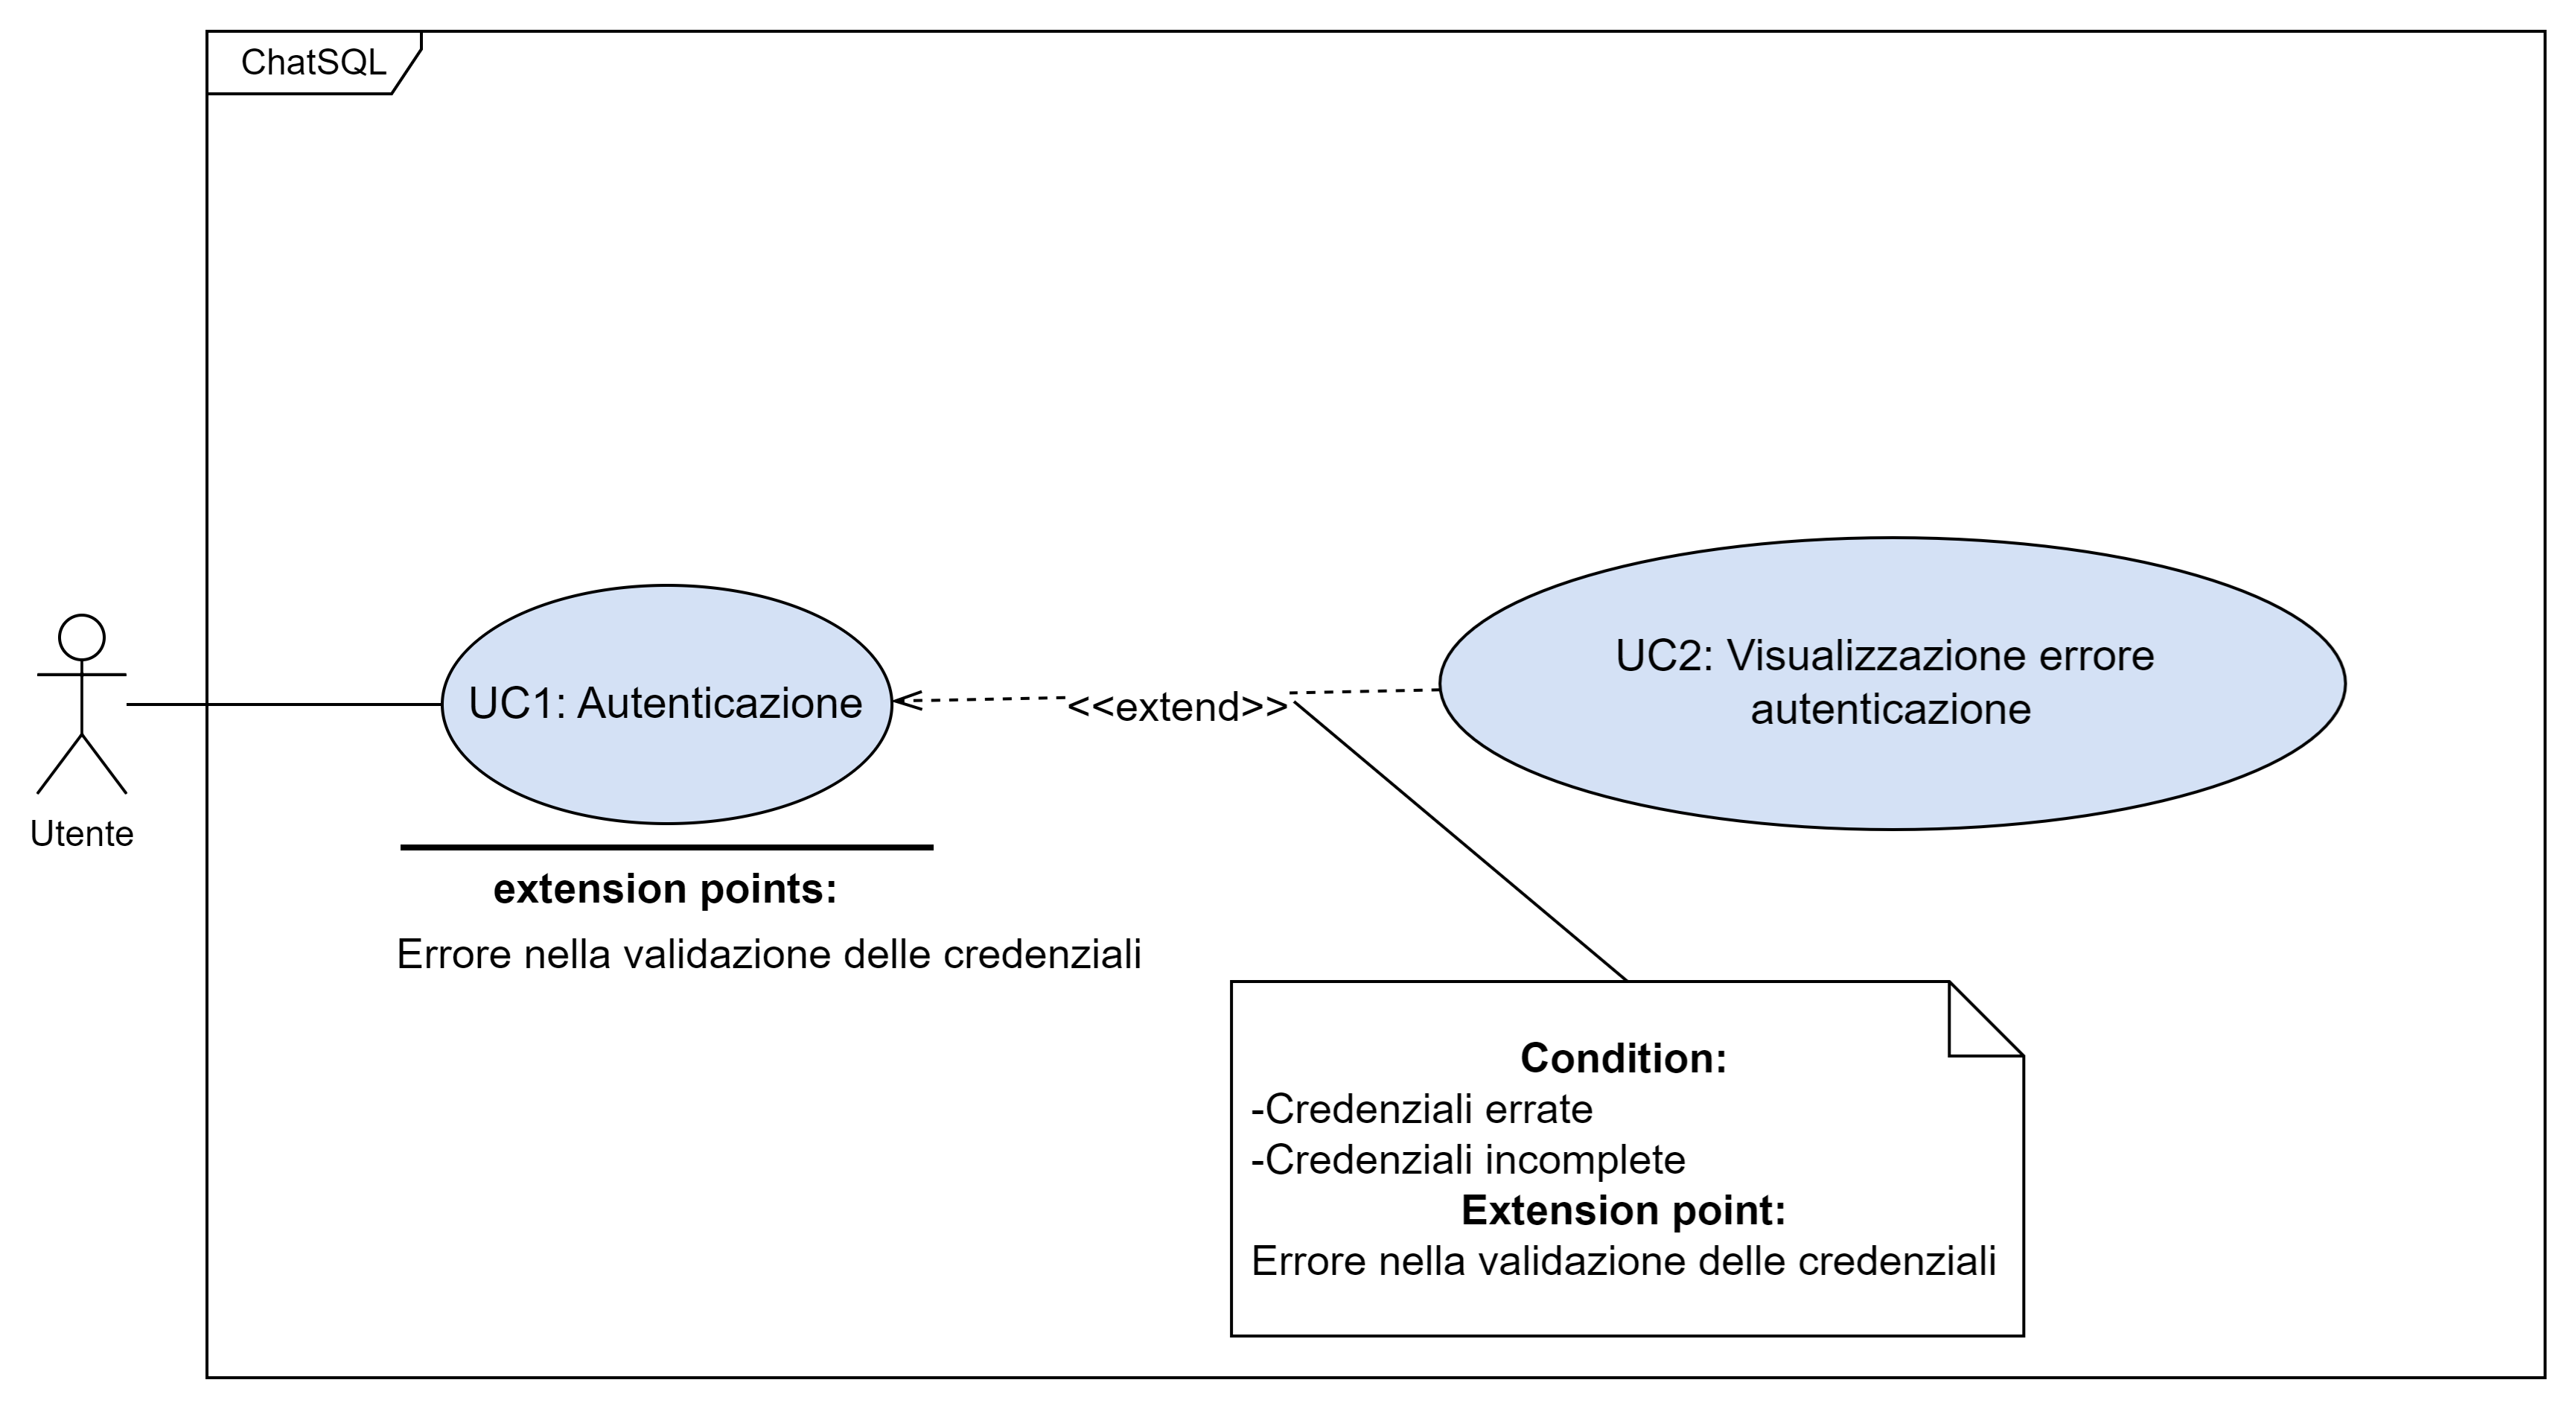
\includegraphics[width=0.95\textwidth]{assets/uc1.png}
  \caption{UC1}
\end{figure}

\paragraph*{Descrizione}
L'autenticazione corrisponde al processo di login, tramite il quale il Tecnico può ampliare le funzionalità disponibili.

\paragraph*{Attori principali}
Tecnico

\paragraph*{Precondizioni}
\begin{itemize}
  \item Il sistema è attivo e funzionante;
  \item Il Tecnico è stato registrato presso il sistema;
  \item Il Tecnico non è autenticato nella sessione corrente.
\end{itemize}

\paragraph*{Postcondizioni}
\begin{itemize}
  \item La procedura di autenticazione si è conclusa con successo;
  \item Il Tecnico visualizza le funzionalità aggiuntive nell'interfaccia.  
\end{itemize}

\paragraph*{Trigger}
Il Tecnico desidera accedere all'area di amministrazione.

\paragraph*{Scenario principale}
\begin{itemize}
  \item Il Tecnico seleziona l'opzione "Login";
  \item Il Tecnico inserisce le proprie credenziali;
  \item Il Tecnico effettua l'accesso;
  \item Il sistema mostra la schermata aggiornata con le funzionalità disponibili.
\end{itemize}

\paragraph*{Scenario alternativo}
\begin{enumerate}
  \item Il sistema riscontra un errore durante la validazione delle credenziali (\hyperref[UC2]{UC2});
  \item Viene visualizzato un messaggio con i dettagli dell'errore.
\end{enumerate}

\paragraph*{Estensioni}
\begin{itemize}
  \item Visualizzazione errore autenticazione (\hyperref[UC2]{UC2}):
  \begin{itemize}
    \item Extension point: Errore nella validazione delle credenziali.
  \end{itemize}
\end{itemize}

\paragraph*{Sottocasi d'uso:}
\begin{itemize}
  \item \hyperref[UC1point1]{UC1.1}: Inserimento username;
  \item \hyperref[UC1point2]{UC1.2}: Inserimento password.
\end{itemize}

\begin{figure}[H]
  \centering
  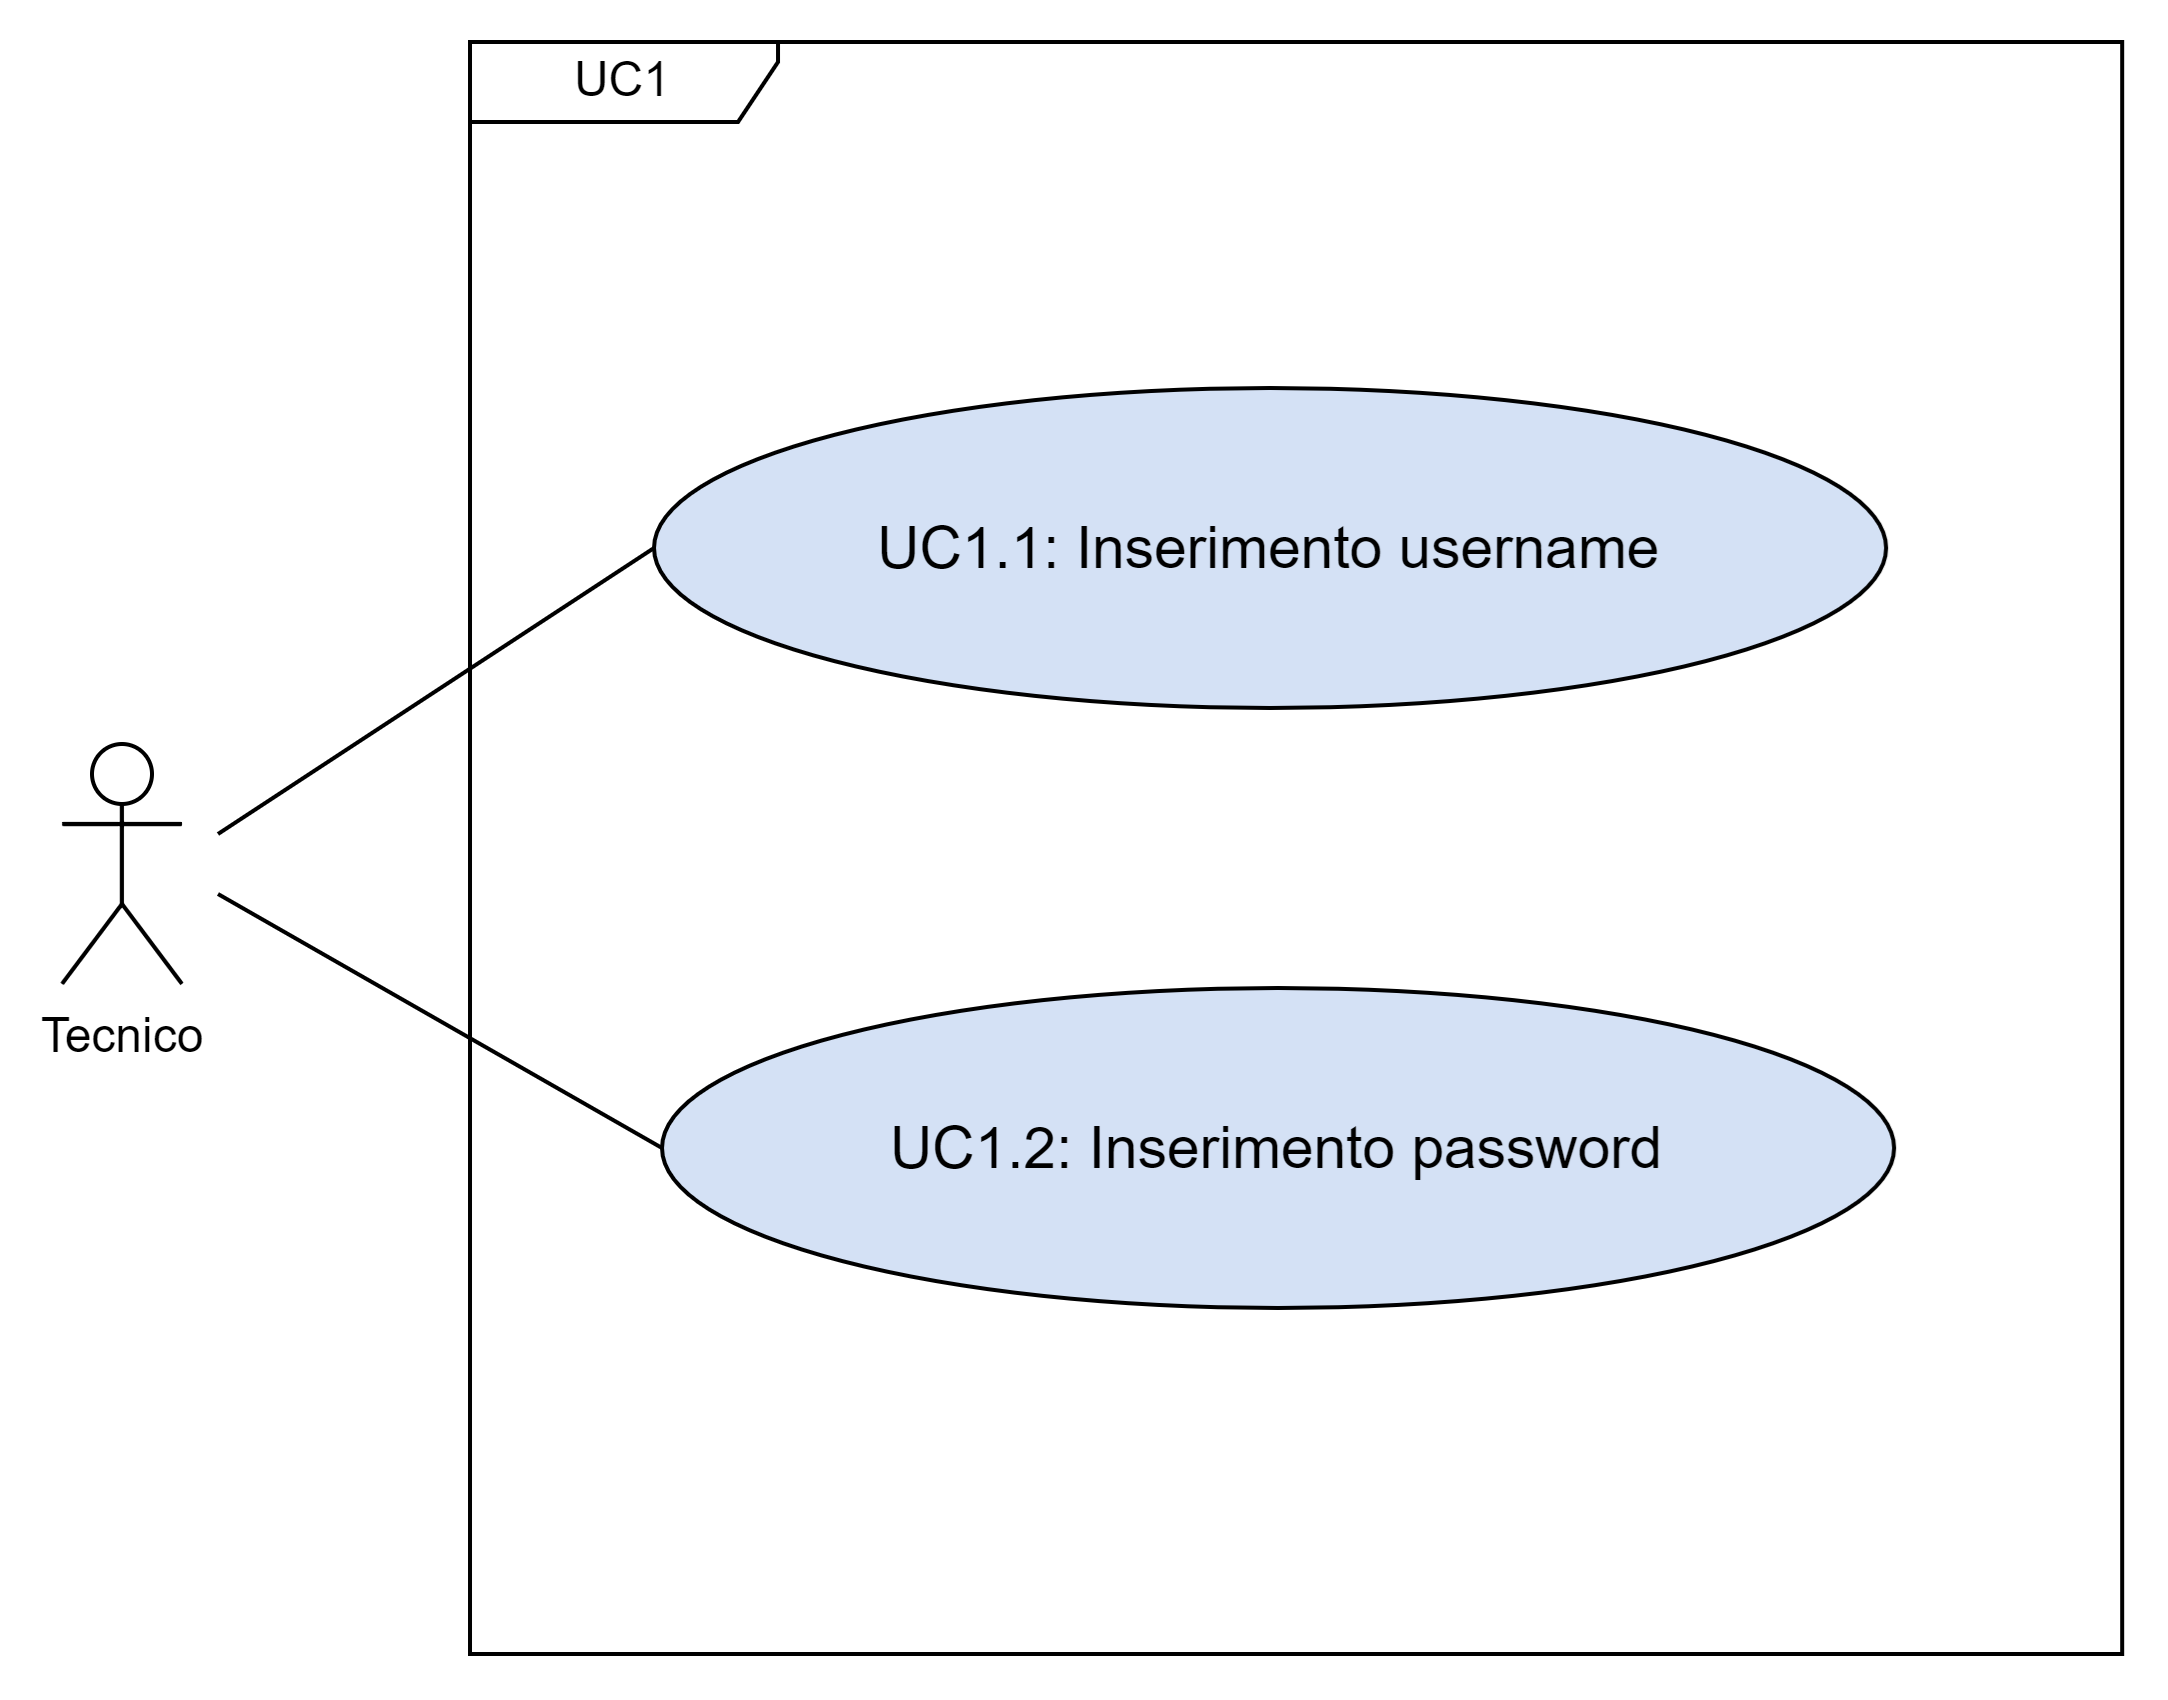
\includegraphics[width=0.80\textwidth]{assets/uc1_1.png}
  \caption{UC1 - Sottocasi d'uso}
\end{figure}

%%%%%%%%%%%%%%%%%%%%%%%%%%%%%%%%%%%%%%%%%%%%%%%%%%%%%%%%%%%%%%%%%%%%%%%%%%%%%%

\subsubsection{UC1.1 - Inserimento username}\label{UC1point1}

\paragraph*{Descrizione}
La procedura di "inserimento username" corrisponde all'immissione del nome utente nella sezione apposita di login.

\paragraph*{Attori principali}
Tecnico

\paragraph*{Precondizioni}
\begin{itemize}
  \item Il sistema è attivo e funzionante;
  \item Il Tecnico ha avviato la procedura di autenticazione (\hyperref[UC1]{UC1}).  
\end{itemize}

\paragraph*{Postcondizioni}
\begin{itemize}
  \item Il nome utente è stato inserito nel campo apposito.
\end{itemize}

\paragraph*{Trigger}
Il Tecnico desidera inserire uno username come parte del processo di autenticazione.

\paragraph*{Scenario principale}
\begin{enumerate}
  \item Il Tecnico inserisce uno username.
\end{enumerate}

%%%%%%%%%%%%%%%%%%%%%%%%%%%%%%%%%%%%%%%%%%%%%%%%%%%%%%%%%%%%%%%%%%%%%%%%%%%%%%

\subsubsection{UC1.2 - Inserimento password}\label{UC1point2}
\paragraph*{Descrizione}
La procedura di "inserimento password" corrisponde all'immissione della password nella sezione apposita di login.

\paragraph*{Attori principali}
Tecnico

\paragraph*{Precondizioni}
\begin{itemize}
  \item Il sistema è attivo e funzionante;
  \item Il Tecnico ha avviato la procedura di autenticazione (\hyperref[UC1]{UC1}). 
\end{itemize}

\paragraph*{Postcondizioni}
\begin{itemize}
  \item La password è stata inserita nel campo apposito.
\end{itemize}

\paragraph*{Trigger}
Il Tecnico vuole inserire una password come parte del processo di autenticazione.

\paragraph*{Scenario principale}
\begin{enumerate}
  \item Il Tecnico inserisce una password.
\end{enumerate}